\documentclass[12pt,twoside]{report}
\setlength\parindent{0pt}
\usepackage[a4paper,width=150mm,top=25mm,bottom=25mm,bindingoffset=6mm]{geometry}
\usepackage[english]{babel}
\usepackage[utf8]{inputenc}
\usepackage[T1]{fontenc}
\usepackage{lmodern}

%Maths Tools
\usepackage{amsmath}
\usepackage{amsthm}
\usepackage{amsfonts}
\usepackage{mathtools}
\usepackage{mathrsfs}
\usepackage{bbold}
\usepackage[overload]{empheq}

\usepackage{hyperref}
\usepackage{lipsum} % Lorem Ipsum
\usepackage{verbatim} % Comments
\usepackage{float}
\usepackage{caption}
\usepackage{subcaption}
\usepackage{setspace}
\usepackage{csquotes}

\usepackage{booktabs, multirow} % for borders and merged ranges
\usepackage{soul}% for underlines
\usepackage[table]{xcolor} % for cell colors
\usepackage{changepage,threeparttable} % for wide tables

\usepackage{tikz}
\usepackage{pgfplots}
\pgfplotsset{compat=1.18}
\pgfplotscreateplotcyclelist{worldlines}{{blue!80!black},{red!80!black},{black},{teal},{orange!90!black},{violet},{brown},{green!50!black},{magenta!80!black},{gray}}
% Worldlines q_1(t), ..., q_N(t) from a CSV file with columns t, q1, ..., qN
% (generated by notebooks/export_figure_data.wls)
\newcommand{\worldlines}[4]{% #1 file, #2 N, #3 width, #4 height
  \begin{tikzpicture}
  \begin{axis}[width=#3, height=#4, xlabel={$t$}, ylabel={$q$},
    enlarge x limits=false, tick label style={font=\footnotesize},
    label style={font=\small}, cycle list name=worldlines,
    every axis plot/.append style={line width=0.6pt, mark=none}]
  \pgfplotsinvokeforeach{1,...,#2}{\addplot table[x=t, y=q##1, col sep=comma]{#1};}
  \end{axis}
  \end{tikzpicture}}
\usepackage{graphicx}

\graphicspath{ {images/} }

\usepackage{fancyhdr}
\pagestyle{fancy}
\setlength{\headheight}{14.5pt}
\fancyhead{}
\fancyhead[RO]{\bfseries \nouppercase \rightmark}
\fancyhead[LE]{\bfseries \nouppercase \leftmark}
\cfoot{\thepage}
\renewcommand{\headrulewidth}{0.4pt}
\renewcommand{\footrulewidth}{0pt}

\usepackage{afterpage}
\newcommand\blankpage{%
    \null
    \thispagestyle{empty}%
    \addtocounter{page}{-1}%
    \newpage}

% Customized environments
\newtheorem{defi}{Definition}
\newtheorem{prop}{Proposition}
\newtheorem{thm}{Theorem}
\newtheorem{cor}{Corollary}
\newtheorem{obs}{Observation}
\newtheorem{lemma}{Lemma}
\newtheorem{example}{Example}

\newcommand{\diag}{\mathop{\mathrm{diag}}}
\DeclareMathOperator{\sech}{sech}

\newenvironment{abstractpage}
  {\cleardoublepage\vspace*{\fill}\thispagestyle{empty}}
  {\vfill\cleardoublepage}
\renewenvironment{abstract}[1]
  {\bigskip\selectlanguage{#1}%
   \begin{center}\bfseries\abstractname\end{center}}
  {\par\bigskip}

\title{\textbf{Soliton solutions to classical Calogero-Moser systems}}
\author{}
\date{}

\makeatletter
\let\inserttitle\@title
\makeatother

\pagenumbering{roman}

\begin{document}

\begin{titlepage}
\begin{center}

\begin{flushleft}
	\begin{minipage}{3.0cm}
	\vspace*{0.7cm}
	\begin{center}
		
\includegraphics[width=3.0cm,height=3.0cm]{images/LogoUnisalento.jpg}
	\end{center}
\end{minipage}\hfill
\end{flushleft}

\vspace*{-25mm}

\begin{minipage}{10cm}
	\begin{center}
    \textsc{\Large Università del Salento}\\[0.3cm]
    \textsc{\large Scuola Superiore ISUFI}\\[0.3cm]
    {\large Curriculum Tecnico-Scientifico}
	\end{center}
\end{minipage}\hfill

\begin{flushright}
 
\vspace*{-31mm}

\begin{minipage}{3.0cm}
	\begin{center}
		
\includegraphics[width=3.0cm,height=3.0cm]{images/LogoISUFI.jpg}
	\end{center}

\end{minipage}
\end{flushright}

\vspace{0.3cm}

\begin{spacing}{0.2}
\rule{\linewidth}{0.4pt}
\rule{\linewidth}{0.4pt}
\end{spacing}

\textsc{\Large }\\[7cm]

% Title
{\Huge {\inserttitle} \\[6cm]}

% Author and supervisor
\noindent
\begin{minipage}{0.4\textwidth}
  \begin{flushleft} \large
    \emph{Mentore:}\\
    Prof. L. \textsc{Martina}\\
  \end{flushleft}
\end{minipage}%
\begin{minipage}{0.5\textwidth}
  \begin{flushright} \large
    \emph{Allievo:} \\
    A. \textsc{Zingarofalo} \\
  \end{flushright}
\end{minipage}\\[1.5cm]

\begin{spacing}{0.2}
\rule{\linewidth}{0.4pt}
\rule{\linewidth}{0.4pt}
\end{spacing}

\vfill

% Bottom of the page
{\large {Anno Accademico}\\ 2021/2022}

\end{center}
\end{titlepage}

\clearpage\pagestyle{empty}\null\newpage

\setcounter{page}{1}
\begin{abstractpage}

\selectlanguage{italian}
\setlocalecaption{italian}{abstract}{Sommario}
\begin{abstract}{italian}

\addcontentsline{toc}{chapter}{Sommario}

 Esponiamo un metodo generale, noto in letteratura, per trovare soluzioni $M$-solitoniche a sistemi classici di Calogero-Moser (CM) di tipo $A_{N-1}$ razionale, iperbolico e trigonometrico, per il generico $M < N$, dove $N$ è il numero di particelle del sistema, tramite trasformazioni di Bäcklund tra sistemi dello stesso tipo. La generalità del metodo è dovuta a una descrizione unificante dei sistemi considerati mediante una speciale funzione di Lax $\alpha(x)$, che genera la rappresentazione di Lax di questi sistemi. \\
 Studiamo numericamente le soluzioni solitoniche per il modello CM razionale con potenziale armonico esterno (eCM) per diversi valori di $N$.
\end{abstract}
\selectlanguage{english}

\begin{abstract}{english}

\addcontentsline{toc}{chapter}{Abstract}

 We review a general method, known from the literature, to find $M$-soliton solutions to the $A_{N-1}$ classical Calogero-Moser (CM) systems of rational, hyperbolic and trigonometric type, for arbitrary $M < N$, where $N$ represents the number of particles of the system, via Bäcklund transformations between systems of the same type. The generality of the method is due to a unifying description of all the systems considered by a special Lax function, which generates the Lax representation of these systems. \\
 We study numerically soliton solutions for the rational CM model with external harmonic potential (eCM) for different values of $N$.

\vspace{1cm}

\emph{Keywords}: integrable systems, Hamiltonian systems, Calogero-Moser systems, \\ \-\ \-\ \-\ \-\ \-\ \-\ \-\ \-\ \-\ \-\ \-\ \-\ \-\ \-\ \-\ \-\ \-\ \-\ \-\ \-\ many-body problem, M-soliton solutions.

%\afterpage{\blankpage}

\end{abstract}
\end{abstractpage}

\setcounter{page}{3}

\tableofcontents

%\afterpage{\blankpage}

\chapter*{Introduction}
\setcounter{page}{5}
\addcontentsline{toc}{chapter}{Introduction}
\markboth{Introduction}{Introduction}
 In this work we will present a method to find $M$-soliton solutions to the classical Calogero-Moser (CM) systems. The CM model has been studied extensively  and occupies a prominent place between integrable systems, a rapidly developing branch of modern mathematical physics and beyond, at the crossroads to many area of mathematics and theoretical physics. \\
 F. Calogero introduced and solved first in a quantum context the 1-dimensional CM system with arbitrary $N$ is \cite{calogero71}. The analogous model on the circle was treated independently by Bill Sutherland in \cite{sutherland}. C. Marchioro studied the classical analogue for the 1-dimensional on the line \cite{marchioro1970, marchioro1974}. In 1975 J. Moser proved that the classical CM system is integrable for arbitrary $N$ (\cite{moser1975}). \\
 In this thesis we will start providing the necessary background of Hamiltonian mechanics in chapter \textsection 1. Then, we will review a few important mathematical tools of modern theory of integrable systems, such as Lax Representation and Bäcklund transformations. In the second chapter we will define the classical Calogero-Moser systems and present some of their properties. We will show how they can be arrived at by means of the Kazhdan-Kostant-Sternberg (KKS) construction and how solutions can be obtained through the Olshanetsky Perelomov (OP) projection method. We will exhibit their Lax representations and their Bäcklund transformations, from which we will derive soliton equations in Chapter \textsection 3.
 We will deal with soliton solutions of systems of Calogero-Moser type. We will define what exactly is a soliton solution to an $N$-body problem and derive them in a unified way for the systems under analysis, following \cite{philip2019soliton}. Lastly, we will study numerically soliton solutions for the rational case with external harmonic potential (hCM) as done by \cite{kulkarni2017, abanov2011}, for different values of $N$.

\chapter{Background: Hamiltonian mechanics}\label{ch:hamiltonian}
\pagenumbering{arabic}
\setcounter{page}{1}
\pagestyle{fancy}
In this chapter we will see some basic concepts of Hamiltonian mechanics: we will define Hamiltonian systems and Poisson brackets, review Hamilton's equations of motion and state some fundamental results concerning integrals of motion in Hamilton's formalism. \\
In the last section we will present some important mathematical tools of modern theory of integrable systems, such as Lax Representation and then Bäcklund transformations, that will play a key role in Chapter \textsection 3.

\section{Hamiltonian systems}
Let us recall some basic elements of Hamiltonian Systems \footnote{For a more complete discussion and insights, please refer to K. Vogtmann, A. Weinstein, and V. Arnol’d, \textit{Mathematical Methods of Classical Mechanics}. Graduate Texts in Mathematics, Springer New York, 1997.}. We start from the definition:

\begin{defi}
A dynamical system of $\;2N$, first order, ordinary differential equations

\begin{equation}
    \dot X = J \nabla \mathcal{H}
\end{equation}

is said an $N$-degree-of-freedom Hamiltonian System if $\mathcal{H}$ the Hamiltonian, is a smooth scalar function defined on the phase space, $\mathcal{H}: \mathcal{T}^\ast \mathcal{M} \to \mathbb{R}$, where $\mathcal{M}$ is a $N$-dimensional smooth manifold (configuration space) and $\mathcal{T}^\ast \mathcal{M}$ its cotangent bundle (\cite{arnold2007mathematical}), and the $N \times N$ antisymmetric matrix

$$J = 
\begin{pmatrix}
0 & \mathbb{1}_N \\
-\mathbb{1}_N  & 0
\end{pmatrix}$$

is called the canonical symplectic matrix, where $\mathbb{1}_N$ is the $N \times N$ identity matrix.
\end{defi}

In its "natural" form, for a system of $N$ particles, one writes

$$\mathcal{H}(q_1,q_2,...,q_N,p_1,p_2,...,p_N) = \sum_{i=1}^N \frac{p_i^2}{2m_i} + V(q_1,q_2,...,q_N)\;.$$

where $q_i$ is the position of the $i^{th}$ particle whose mass is $m_i$ , and $p_i$ is its canonical momentum $p_i = m_i \dot q_i$ . The equations of motion are

\begin{equation}
\dot q_i = \frac{\partial \mathcal{H}}{\partial p_i}\;\;\;\;, \;\;\;\;
\dot p_i = - \frac{\partial \mathcal{H}}{\partial q_i}\;,
\end{equation}

which are equivalent to Newton's equation of motion. 

\begin{defi}
We define the Poisson brackets for any couple of functions $F(q,p)$ and $G(q,p)$ on the phase space as follows:

\begin{equation}
    \{F, G\} = \sum_{i=1}^N \Big (\frac{\partial F}{\partial q_i}\frac{\partial G}{\partial p_i} - \frac{\partial F}{\partial p_i}\frac{\partial G}{\partial q_i} \Big )\;.
\end{equation}
\end{defi}

\begin{prop}
Let $A$, $B$, $C: \mathcal{T}^\ast \mathcal{M} \to \mathbb{R}$, $k$, $h \in \mathbb{R}$. The Poisson brackets obey the following properties:

\begin{enumerate}
\item $\{A, B\} = - \{B, A\}$ (antisymmetry);
\item $\{A, kB + hC\} = k\{A, B\} + h\{A, C\}$ (bilinearity);
\item $\{A, BC \} = \{A, B\}C + B\{A, C \}$ (Leibniz rule);
\item $\{A, \{B, C \}\} + \{B, \{C ,A\}\} + \{C , \{A, B\}\} = 0$ (Jacobi identity).
\end{enumerate}
\end{prop}

If $\delta_{ij}$ denote the Kronecker delta, the coordinates $(q_1, ..., q_n, p_1, ..., p_n)$ satisfy canonical relations:

\begin{equation}
    \{q_i, q_j\} = \{p_i, p_j\} = 0, \;\;\;\;\;\; \{p_i, q_j\} = \delta_{ij}\;.
\end{equation}

It yields the following

\begin{thm}
A function $F$ on phase space, $F:\mathcal{T}^\ast\mathcal{M} \to \mathbb{R}$ is a first integral for the Hamiltonian system $\mathcal{H}$ if and only if 

\begin{equation}
    \{F, \mathcal{H}\} = 0\;.
\end{equation}
\end{thm}

\section{Canonical and Bäcklund transformations}
\subsection{Canonical transformations}
A natural question is which are the transformations that leave invariant in form the Hamilton equations. Such transformations are called \textit{canonical}.

\begin{defi}
The coordinate transformation $T$

\begin{equation}
    T: \left \{ \begin{array}{cc}
    q = & q(\tilde q, \tilde p) \\
    p = & p(\tilde q, \tilde p)
\end{array}
\right.
\end{equation}

is said to be canonical if, however the Hamiltonian $\mathcal{H}: \mathcal{T}^\ast \mathcal{M} \to \mathbb{R}$ is taken, the Hamiltonian equations

\begin{equation}
\dot q = \frac{\partial \mathcal{H}}{\partial p}\;\;\;\;, \;\;\;\;
\dot p = - \frac{\partial \mathcal{H}}{\partial q}
\end{equation}

are equivalent to the new equations

\begin{equation}
\dot{\tilde q} = \frac{\partial \tilde{\mathcal{H}}}{\partial \tilde p}\;\;\;\;, \;\;\;\;\dot{\tilde p} = - \frac{\partial \tilde{\mathcal{H}}}{\partial \tilde q}\;,
\end{equation}

where $\tilde{\mathcal{H}} = \mathcal{H} \circ T$, i.e. $\tilde{\mathcal{H}}(\tilde q, \tilde p) = \mathcal{H}(T(q,p))$.
\end{defi}

\begin{defi}
A coordinate transformation $T$ 

\begin{equation}
    T: (q,p) = T(\tilde q, \tilde p)
\end{equation}

preserves the Poisson brackets. If two functions on phase space $F$ and $G$ are defined, denoting by $\tilde F = F \circ t$, $\tilde G = G \circ t$ the transformed functions, it results 

\begin{equation}
    \{\tilde F, \tilde G\} = \{F, G\} \circ T\;.
\end{equation}
\end{defi}

\subsection{Hamiltonian Bäcklund transformations}
A subset of canonical transformations is made up by the Hamiltonian Bäcklund transformations (more precisely Hamiltonian auto-Bäcklund transformations), which will play a crucial role in the search for soliton solutions. \\
A \textit{Bäcklund transformation} (BT) between a pair of differential equations

\begin{equation}
    P(u) = 0\;\;\;\;,\;\;\;\;Q(v) = 0\;,
\end{equation}

maps solutions of one to solutions of the other. They were introduced in 1880 by A. V. Bäcklund \cite{backlund1880} in a differential geometry context, as a map between 3-dimensional surfaces. \\
In the large part of the literature, the term \textit{Bäcklund transformations} refers to \textit{auto-Bäcklund transformations} \cite{philip2019soliton}, in the sense that the two equations coincide: $P \equiv Q$.\\
An \textit{auto-Bäcklund transformation} is a transform that leaves a partial differential equation invariant. It can also provide a method whereby a known solution to a partial differential equation can be transformed into a different solution to the same PDE. This solution can then be used to obtain a new solution. \\
By naturally declining the definition for Hamiltonian systems, an Hamiltonian auto-Bäcklund transformation is a map between canonical coordinates, $(x(t), \dot x(t)) \to (z(t), \dot z(t))$ that leaves Hamilton's equations invariant. 
As already mentioned, Hamiltonian auto-Bäcklund transformations belong to a subset of canonical transformations, with the special property of preserving the Hamiltonian function \cite{kuznetsov1998}.

\begin{example}
    The well known Cauchy-Riemann conditions
    
    \begin{equation}
        \left \{ \begin{array}{cc}
        u_x - v_y &= 0 \\
        u_y + v_x &= 0
        \end{array}
        \right.
    \end{equation}
    
    are examples of auto-Bäcklund transformations connecting different solutions $u(x,y), v(x,y)$ to the Laplace equation $\nabla^2 w(x,y) = 0$.
\end{example}

\section{Integrable systems}
\subsection{Introduction to integrability}
A standard way to investigate the behavior of a physical system is to construct a mathematical model of the system, solve the model, use it to make predictions and compare theoretical results with experiments. However, often the differential equations provided by these models cannot be solved analytically and solutions can only be approximated numerically. Relatively few systems, however, can be solved exactly with explicit analytic expressions. These systems are called "integrable". \\
The field of integrable systems is born together with Classical Mechanics \cite{babelon2003}, with a quest for exact solutions to Newton's equations of motion \cite{newton1687}. After two centuries from Newton's solution of the Kepler problem, only a few other cases were found:

\begin{itemize}
    \item geodesics on ellipsoid (Jacobi, 1837, \cite{jacobi1936});
    \item the harmonic oscillator on the sphere (Neumann, 1859, \cite{neumann1859});
    \item Lagrange, Euler and Kovalevskaya \cite{kowalevski1889} tops.
\end{itemize}

We need to clarify that the concept of integrability is not the same as resolubility. There are integrable systems that cannot be expressed analytically, just as there are systems exactly solvable that are not integrable. Solvability ultimately depends on capacity and computational power. Integrability refers rather to the property of a system to exhibit regular behaviors (quasi-periodic) for every possible condition initial condition, as opposed to chaotic and irregular ones. For this reason, an inclusive definition of integrable system is elusive, as repeatedly pointed out in \cite{zakharov2012integrability}.

\subsection{Action-Angle variables}
Consider an autonomous Hamiltonian system with $N$ degrees of freedom, of Hamiltonian $\mathcal{H}(q, p)$; with evidence if $\mathcal{H}$ does not depend on one or more coordinates, e.g. $q_{M+1}, . . . , q_N$, $0 \leq M < N$, then the corresponding conjugate moments $p_{M+1}, . . . , p_N$ are constants of the motion of the system, and in practice the Hamiltonian system with $N$ degrees of freedom is reduced to a system with only $M$ degrees of freedom. If then $\mathcal{H}$ is independent of all coordinates $q_1, . . . , q_N$, that is, we have $\mathcal{H}(q, p) = h(p)$, then the integration of the equations of motion is completely trivial: in fact, posited $\omega_i(p) = \frac{\partial h}{\partial p_i}$ , $i = 1, . . . , N$, the equations of motion become $\dot p_i = 0, \dot q_i = \omega_i(p)$, and thus the general integral is written

\begin{equation}
p_i(t) = p_i^0 \;\;\;\;,\;\;\;\; q_i(t) = q_i^0 + \omega_i(p^0)t ,\; , \end{equation}

where $q_i^0$ , $p_i^0$ , $i = 1, . . . , N$, denote the initial data.
The motion in the new variables then takes place on a torus $\mathbb{T}^N$ and is linear:

\begin{equation}
    I(t) = I_0\;\;\;\; , \;\;\;\;\phi(t) = \phi_0 + \omega(I_0)t
\end{equation}

with $\omega = \frac{\partial h}{\partial I}$, and in the new variables the phase space appears naturally decomposed into the product $B \times \mathbb{T}^N$. For their geometric interpretation, these variables $(I, \phi)$ are called action-angle variables. \\
We can now 

\begin{defi}
The Hamiltonian $\mathcal{H} : D \to \mathbb{R}$ is said to be integrable according to Liouville in the domain $D' \subset D$
if there exists a canonical transformation $(q, p) = T(I, \phi)$, defined for $I \in B \subset \mathbb{R}^n$ and $\phi \in \mathbb{T}^N$, such that

\begin{enumerate}
\item $D' = T(B \times \mathbb{T}^N)$, 
\item the new Hamiltonian $\tilde{\mathcal{H}} = \mathcal{H} \circ T$ is a function of actions only:

$$\tilde{\mathcal{H}}(I, \phi) = h(I)\;\;\;\;,\;\;\;\; h : B \to \mathbb{R} \;.$$
\end{enumerate}
\end{defi}

In the second half of the nineteenth century, J. Liouville  \cite{Liouville1855} provided a general criterion characterizing the cases where the equations of motion are “solvable by quadratures”. This result was reported by V. I. Arnol'd in \cite{arnold1997} with a new proof based on symplectic geometry. This contribution was so important that now the theorem is known as the Liouville-Arnol'd theorem:

\begin{thm}[Liouville-Arnol'd]
If a Hamiltonian system with $n$ degrees of freedom has $N$ integrals of motion $\mathcal{H}_1, \mathcal{H}_2, ..., \mathcal{H}_N$, ($\mathcal{H}_i:\mathcal{T}^\ast \mathcal{M} \to \mathbb{R}\;\forall i = 1,...,N$ ):
\begin{enumerate}
\item functionally independent and analytical in their variables,
\item in involution, i.e. $\{\mathcal{H}_i, \mathcal{H}_j\} = 0 \;\forall i \neq j$,
\end{enumerate}
then the system can be integrated by quadratures.
\end{thm}

\subsection{Lax representation of an integrable system}
A new concept emerged from modern studies on integrable systems is the notion of Lax pairs \cite{lax1968}, introduced by the Hungarian-born American mathematician Peter Lax in 1968.

\begin{defi}
A Lax pair $(L,M)$ consists of two square matrices, functions on the phase space of the system, such that the Hamiltonian evolution equations may be written as

\begin{equation}\label{laxevolution}
\dot L = [L, M]
\end{equation}

where $[L,M]$ denotes the commutator on the set of matrices. 
\end{defi}

Suppose that $\mathcal{H}$ is integrable, and that the integrals of motion $\mathcal{H}_1, ..., \mathcal{H}_N$ are known. Then

$$ \hat L = \diag{ \{\mathcal{H}_i : i=1,...,N \}} $$

is the Lax representation of $\mathcal{H}$. Note that $\mathcal{H}_1, ..., \mathcal{H}_N$ are the eigenvalues of $\hat L$. \\
Because similarity transformations preserve eigenvalues, if

$$L = U \hat LU^{-1}$$

where $U(t)$ is some invertible matrix, then the eigenvalues $\lambda_i$ of $L$ coincide with the ones of $\hat L$: $\lambda_i = \mathcal{H}_i$ ($i=1, ..., n$). Consider now the eigenvalue equation

$$Lu_i = \lambda_i u_i\;.$$

Taking the time derivative we get:

$$\dot L u_i + L \dot u_i = \dot \lambda_i u_i + \lambda_i \dot u_i = \lambda_i \dot u_i\;.$$

Supposing $\dot u_i = - M u_i$, where $M \in \mathbb{C}^{\;N\times N}$ we have

$$\dot L u_i - LMu_i = -\lambda_i M u_i = - M \lambda_i u_i = - MLu_i\;,$$

thus

$$\dot L u_i - LMu_i = -MLu_i \iff (\dot L - [L,M])u_i = 0\;\;.$$

which implies

$$\dot L = [L,M]\;.$$

Since the elements of $L$ are functions on phase space, the Lax evolution equations must be equivalent to Hamilton's equations of motion for $\mathcal{H}$.

\begin{thm}
Given a Lax pair $(L,M)$ for a dynamical system, then the functions

\begin{equation}
tr(L^k)\;\;\;\;,\;\;\;\;k = 1, 2, ..., 
\end{equation}

are all the integrals of motion of the dynamical system.
\end{thm}

\begin{proof}
    For $k=1$ we have
    
    $$\frac{d}{dt} tr(L) = tr(\dot L) = tr(LM - ML) = 0$$
    
    due to the cyclic property of the trace operator. More generally
    
\begin{equation*}
\begin{split}
\frac{d}{dt}L^k &= \dot L L^{k-1} + L\dot L L^{k-2} + ... + L^{k-2} \dot L L + L^{k-1} \dot L = \\
&= LML^{k-1} - ML^k -LML^{k-1} + L^2ML^{k-2} + ...\\
&\; - L^{k-2}ML^2 + L^{k-1}ML - L^{k-1}ML + L^k M = \\
&= [L^k , M] \;.
\end{split}
\end{equation*}
    
    Then
    $$\frac{d}{dt} tr(L^k) = tr(\frac{d}{dt} L^k) = tr(L^k M - ML^k) = 0\;.$$
\end{proof}

\begin{example}
A Lax pair for the harmonic oscillator has the form:

$$L = 
\begin{pmatrix}   
p & \omega q\\   
\omega q & -p  
\end{pmatrix},\;\;\;
M = 
\begin{pmatrix}   
0 & \frac{\omega}{2}\\   
-\frac{\omega}{2} & 0  
\end{pmatrix}\;.$$

The characteristic equation

\begin{equation}
    (p-\lambda) (p + \lambda) + \omega^2 q^2 = 0
\end{equation}

gives the eigenvalues

\begin{equation}
    \lambda_{1,2} = \pm \sqrt{p^2 + \omega^2 q^2}\;,
\end{equation}

that are integrals of motion of the system related to the energy. \\
We check immediately that the Lax evolution equation, $\dot L = [L, M]$, is equivalent to the equations of motion

$$\dot q = p, \;\;\;\;\;\;\;\;\dot p = -\omega^2 p\;\;\,.$$
\end{example}

\chapter{Calogero-Moser systems}\label{ch:cm}
In this chapter we will present the classical Calogero-Moser systems under consideration and some of their properties. We will show how they can be arrived at by means of the Kazhdan-Kostant-Sternberg (KKS) construction and how solutions can be obtained through the Olshanetsky-Perelomov (OP) projection method. Lastly, we will report their Lax representations and their Bäcklund transformations, from which we will derive soliton equations in Chapter~\ref{ch:solitons}.


\section{Calogero-Moser (CM) systems}

\begin{defi}
Let $(q, p) = (q_1, \dots, q_N, p_1, \dots, p_N)$ be a set of canonical coordinates. A dynamical system is said to be an $A_{N-1}$ Calogero-Moser \textnormal{(CM)} system with some external potential $W(x)$ if it is characterized by the Hamiltonian

\begin{equation}
\mathcal{H}_{CM} = \sum_{i=1}^N \Big(\frac{1}{2} p_i^2 + W(q_i)\Big) + g^2 \sum_{1 \leq i < j \leq N} V(q_i - q_j)\;,
\end{equation}

(with unit masses), where $g^2$ is the coupling constant and the interparticle potential $V (x)$ belongs to the classified set of meromorphic functions

\[V(x) = \left \{ \begin{array}{ccc}
{1}/{x^2} & \textnormal{(rational)} & \textnormal{(I)}\\
{a^2}/{\sin^2{ax}} & \textnormal{(trigonometric)} & \textnormal{(II)}\\
{a^2}/{\sinh^2{ax}} & \textnormal{(hyperbolic)} & \textnormal{(III)}\\
\wp (x) & \textnormal{(elliptic)} & \textnormal{(IV)}
\end{array}
\right.\]

where $\wp (x)$ is the \textit{elliptic, doubly periodic Weierstrass function}

\begin{equation}
    \wp (z, \omega_1, \omega_2) = \frac{1}{z^2} + \sum_{m, n \neq (0,0)} \Big (  \frac{1}{(z - 2m\omega_1 - 2n\omega_2)^2} - \frac{1}{(2m\omega_1 + 2n\omega_2)^2}\Big )
\end{equation}

with periods $2\omega_1$ and $2\omega_2$.
\end{defi}

These forms of the potential are not arbitrary. They are fixed by the form of the Lax pair proposed by F. Calogero (see Section~\ref{laxcouples}). The equivalence between the equations of motion and the Lax evolution equation puts strong constraints on Calogero's ansatz, which result in the functional equation (\ref{laxfunctionalequations}) for the Lax function. Its general solution is given in terms of the Weierstrass elliptic function $\wp(x)$ (see \cite{calogero2003classical} for a detailed derivation). In fact, the type I-III systems can be viewed as limiting cases of the type IV system \cite{ruijsenaars1999systems}:

\begin{equation}
    \wp(x) = \left \{ \begin{array}{ccc}
    {1}/{x^2} & \omega_1 = \infty & \omega_2 = \infty\\
    {a^2}/{\sin^2{ax}} - {a^2}/{3} & \omega_1 = {\pi} / {2a} & \omega_2 = i\infty\\
    {a^2}/{\sinh^2{ax}} + {a^2}/{3} & \omega_1 = \infty\ & \omega_2 = {i\pi}/{2a}
\end{array}
\right.
\end{equation}

More generally, the potential $V(x)$ is constructed from root systems of Lie algebras, as reported in \cite{perelomov1989}. \\
From Hamilton's equations we get the equation of motion of the $i^{\textnormal{th}}$ particle

\begin{equation}
    \ddot q_i = - W'(q_i) - g^2 \sum_{j = 1,\;j \neq i}^N V'(q_i - q_j)\;,
\end{equation}

where we used that $V$ is even. In this work, we will deal with the classical CM systems I, II and III. We will also consider the rational Calogero-Moser system with external harmonic potential, $W(x) = \frac{1}{2}\omega^2 x^2$, denoted by $\textnormal{I}^+$ or eCM.

\section{KKS construction of CM systems}
Given a dynamical system with a Hamiltonian $\mathcal{H}:\mathcal{T}^\ast \mathcal{M} \to \mathbb{R}$ invariant under a continuous 1-parametric symmetry group, Noether’s theorem \cite{noether1918} gives rise to integrals of motion corresponding to this symmetry. The procedure of \textit{Hamiltonian reduction} consists in eliminating some degrees of freedom by setting these integrals to constant values. In this way we are able to obtain a new submanifold, $\mathcal{T}^\ast \mathcal{M}_{red}$ of lower dimension than the initial one, usually simplifying the problem\footnote{For a more formal treatment, see V.~I. Arnold, V.~V. Kozlov and A.~I. Neishtadt, \textit{Mathematical Aspects of Classical and Celestial Mechanics}, 3rd ed., Encyclopaedia of Mathematical Sciences, Springer, Berlin, 2007, in particular Section 3.2.2, pp.~116--120.}.
In this case, the reduced Hamiltonian typically is more complicated than the original one, suggesting in reverse to construct a system with more degrees of freedom where the hidden symmetries are apparent. \\
In the Kazhdan-Kostant-Sternberg (KKS) construction of CM systems \cite{KKS1978}, CM systems emerge from Hamiltonians on the larger configuration space $X^0_N = \{X\}$ of $N \times N$ Hermitian matrices $X$. We set the phase manifold as the cotangent bundle $\mathcal{T}^\ast X^0_N$, mapped by canonical pairs of $N \times N$ matrices $(X,Y)$. The new system is chosen to be dynamically simple, so that its equation of motion can be solved in closed form \cite{perelomov1989}. \\
If $U$ is a unitary $N \times N$ matrix, then the Hamiltonians are invariant with respect to similarity transformations

\begin{equation}
    (X, Y) \mapsto (UXU^{-1}, UYU^{-1})\;.
\end{equation}

Let us introduce the following $N \times N$ Hermitian matrices:

\begin{equation}
\begin{cases}
Q_{nm} = \delta_{nm} q_n(t) \\
L_{nm} = \delta_{nm}p_n(t) + (1 - \delta_{nm}) \frac{ig}{q_n - q_m}\;.
\end{cases}
\end{equation}

Such matrices are made to correspond to generic Hermitian matrices $X, Y \in X_N^0$ (see \cite{olshanetskyperelomov} for details) by a similarity transformation that leaves the Hamiltonian of the system invariant:

\begin{equation}
    X = UQU^{-1}\;\;\;\;,\;\;\;\;Y = ULU^{-1}\;.
\end{equation}

We report below the construction for each of the cases under analysis.

\subsection{Rational CM (rCM) system}
The KKS construction of the rational CM system leads to the Hamiltonian

\begin{equation}
    \mathcal{H}_{rCM} = \frac{1}{2}\operatorname{tr}(Y^2), \;\;\;\;\;\;(X,Y) \in \mathcal{T}^\ast X^0_N
\end{equation}

describing free motion on $X^0_N$. Applying the similarity transformation we get

\begin{equation}
    \mathcal{H}_{rCM} = \frac{1}{2}\operatorname{tr}(Y^2) = \frac{1}{2}\operatorname{tr}(UU^{-1}Y^2) = \frac{1}{2}\operatorname{tr}(U^{-1} Y^2 U) = \frac{1}{2}\operatorname{tr}(L^2)\;.
\end{equation}

It is easy to verify that the projection $X \to Q$, $Y \to L$ reduces the system to the rCM one:
    
\begin{equation}
    \mathcal{H}_{rCM} = \frac{1}{2}\operatorname{tr}(L^2) = \frac{1}{2}\sum_{i=1}^N p_i^2 + g^2 \sum_{1 \leq i < j \leq N} \frac{1}{(q_i - q_j)^2}\;.
\end{equation}

\subsection{Rational CM system with external harmonic potential (eCM)}
The KKS construction of the rational CM system with external harmonic potential starts from the Hamiltonian

\begin{equation}
    \mathcal{H}_{eCM} = \frac{1}{2}\operatorname{tr}(Y^2 + \omega^2 X^2), \;\;\;\;\;\;(X,Y) \in \mathcal{T}^\ast X^0_N\;,
\end{equation}

describing harmonic motion on $X^0_N$.

Applying the same similarity transformation we get

\begin{equation}
\begin{split}
    \mathcal{H}_{eCM} &= \frac{1}{2}\operatorname{tr}(Y^2) + \frac{1}{2}\omega^2 \operatorname{tr}(X^2) = \\  &= \frac{1}{2}\operatorname{tr}(UU^{-1}Y^2) + \frac{1}{2}\omega^2 \operatorname{tr}(UU^{-1} X^2) = \\ 
    & = \frac{1}{2}\operatorname{tr}(U^{-1} Y^2 U) + \frac{1}{2}\omega^2 \operatorname{tr}(U^{-1} X^2 U)= \frac{1}{2}\operatorname{tr}(L^2) + \frac{1}{2}\omega^2 \operatorname{tr}(Q^2)\;.
\end{split}
\end{equation}

The projection then gives
    
\begin{equation}
    \mathcal{H}_{eCM} = \frac{1}{2}\operatorname{tr}(L^2) + \frac{1}{2}\omega^2 \operatorname{tr}(Q^2)= \frac{1}{2}\sum_{i=1}^N (p_i^2 + \omega^2 q_i^2) + g^2 \sum_{1 \leq i < j \leq N} \frac{1}{(q_i - q_j)^2}\;.
\end{equation}


\subsection{Trigonometric CM (tCM) system}
The trigonometric CM system derives from the Hamiltonian on $\mathcal{T}^\ast X^0_N$

\begin{equation}
    \mathcal{H} = \frac{1}{2}\operatorname{tr}((XY)^2), \;\;\;\;\;\;(X,Y) \in \mathcal{T}^\ast X^0_N\;.
\end{equation}

By applying the previous map we obtain

\begin{align*}
\mathcal{H} &= \frac{1}{2}\operatorname{tr}((XY)^2)=\frac{1}{2}\operatorname{tr}(UU^{-1}XUU^{-1}YUU^{-1}XUU^{-1}Y) = \\
&= \frac{1}{2}\operatorname{tr}(U^{-1}YUU^{-1}XUU^{-1}YUU^{-1}XU) = \frac{1}{2}\operatorname{tr}(QLQL) = \frac{1}{2}\operatorname{tr}((QL)^2)\;.
\end{align*}

Carrying out the calculations, we recover

\begin{equation}
\mathcal{H} = \frac{1}{2} \sum_{i=1}^N q_i^2 p_i^2 + g^2 \sum_{1 \leq i < j \leq N} \frac{q_i q_j}{(q_i - q_j)^2}\;.
\end{equation}

Here $X$ is unitary, so its eigenvalues lie on the unit circle. Then, with the canonical transformation

\begin{equation}
    \begin{cases}
    q_i = e^{2ia\hat q_i} \\
    \hat p_i = 2ia\, q_ip_i
    \end{cases}
\end{equation}

we have $q_i q_j/(q_i - q_j)^2 = -1/(4\sin^2{a(\hat q_i - \hat q_j)})$, and we get

\begin{equation}
\mathcal{H} = -\frac{1}{4a^2}\Big(\frac{1}{2} \sum_{i=1}^N \hat p_i^2 + g^2 \sum_{1 \leq i < j \leq N} \frac{a^2}{\sin^2{a(\hat q_i - \hat q_j)}}\Big) = -\frac{1}{4a^2}\,\mathcal{H}_{tCM}\;.
\end{equation}

The constant factor only rescales time, so the dynamics is that of the trigonometric CM system.

\subsection{Hyperbolic CM (hCM) system}
The hyperbolic CM system derives from the Hamiltonian on $\mathcal{T}^\ast X^0_N$

\begin{equation}
    \mathcal{H} = \frac{1}{2}\operatorname{tr}((XY)^2), \;\;\;\;\;\;(X,Y) \in \mathcal{T}^\ast X^0_N\;.
\end{equation}

which is the same Hamiltonian as in the trigonometric case, but now $X$ is a positive-definite Hermitian matrix. Operating in the same way as above, with the canonical transformation $q_i = e^{2a\hat q_i}$, $\hat p_i = 2a\, q_ip_i$, we have $q_i q_j/(q_i - q_j)^2 = 1/(4\sinh^2{a(\hat q_i - \hat q_j)})$, and we obtain

\begin{equation}
    \mathcal{H} = \frac{1}{4a^2}\Big(\frac{1}{2} \sum_{i=1}^N \hat p_i^2 + g^2 \sum_{1 \leq i < j \leq N} \frac{a^2}{\sinh^2{a(\hat q_i - \hat q_j)}}\Big) = \frac{1}{4a^2}\,\mathcal{H}_{hCM}\;.
\end{equation}

\section{The Olshanetsky-Perelomov (OP) projection method}
Integrating the equations of motion of these systems directly is hard. However, an alternative method of integration has been developed by M. A. Olshanetsky and A. M. Perelomov in \cite{olshanetskyperelomov}. Their projection method amounts to the integration of the auxiliary Hamiltonian systems, from which the solution to the considered ones can be recovered by projection.

\subsection{Rational CM system}
From free motion on $X^0_N$, described by the Hamiltonian

\begin{equation}
    \mathcal{H} = \frac{1}{2}\operatorname{tr}(Y^2), \;\;\;\;\;\;(X,Y) \in \mathcal{T}^\ast X^0_N\;.
\end{equation}

we obtain the equation of motion $\ddot X = 0$, which integrates directly to 

\begin{equation}
    X = At + B\;\;\;\;,\;\;\;\;A, B \in X^0_N\;.
\end{equation}

Given a similarity transformation

\begin{equation}
    X(t) = U(t) Q(t) U^{-1}(t)
\end{equation}

where $U$ is a unitary $N \times N$ matrix, we differentiate with respect to time, obtaining

\begin{equation}
    \dot X = A = \dot UQU^{-1} + U \dot Q U^{-1} + UQ \dot U^{-1}\;
\end{equation}

Since $\dot U^{-1} = - U^{-1} \dot U U^{-1}$,

\begin{equation}
    \dot X = \dot UQU^{-1} + U \dot Q U^{-1} -UQU^{-1}\dot U U^{-1}\;.
\end{equation}

Then, with some algebraic manipulations, 

\[\dot X = UU^{-1}\dot UQU^{-1} + U \dot Q U^{-1} -UQU^{-1}\dot U U^{-1} = 
    U(U^{-1} \dot U Q + \dot Q - QU^{-1} \dot U )U^{-1}\;.\]

Let $M = U^{-1}\dot U$, then

\begin{equation}
    \dot X = U(MQ + \dot Q - QM)U^{-1} = U(\dot Q - [Q, M])U^{-1} = A\;.
\end{equation}

Now, let $L = \dot Q - [Q,M]$, the previous expression becomes

\begin{equation}
    \dot X = ULU^{-1} = A.
\end{equation}

Differentiating again with respect to time, we get

\begin{equation*}
\begin{split}
\ddot X = 0 &= \dot ULU^{-1} + U\dot L U^{-1} + UL\dot U^{-1} =\\
 &= UU^{-1}\dot ULU^{-1} + U\dot L U^{-1} - ULU^{-1}\dot U U^{-1} =\\
&= U(ML + \dot L- LM)U^{-1}\;.
\end{split}
\end{equation*}

Hence, 

\begin{equation}
    \ddot X = U(\dot L - [L,M])U^{-1} = 0\;.
\end{equation}

We observe that, given an $M$, the matrix $U(t)$ is defined up to initial value by $M = U^{-1}\dot U \iff \dot U = UM$. Setting $U(0) = \mathbb{1}_N$, the previous relations allow us to determine $A$ and $B$:

\begin{equation}
    \dot X = A = U(t)L(t)U^{-1}(t) = U(0)L(0)U^{-1}(0) = \mathbb{1}_N L(0) \mathbb{1}_N = L(0)\;,
\end{equation}

\begin{equation}
    X(0) = B = U(0)Q(0)U^{-1}(0) = \mathbb{1}_N Q(0) \mathbb{1}_N = Q(0)\;.
\end{equation}

Consequently

\begin{equation}
    X(t) = At + B = L(0)t + Q(0)\;,
\end{equation}

completely determining $X$ as

\begin{equation}
    X_{nm} (t) = \delta_{nm} (p_n(0)t + q_n(0)) + (1 - \delta_{nm}) ig \frac{t}{q_n(0) - q_m(0)}\;,
\end{equation}

that represents the solution to the equation of motion $\ddot X = 0$ on $X^0_N$. Finally, the time evolution of $Q(t)$ is given by

\begin{equation}
    Q(t) = U^{-1}(t) X(t) U(t)\;.
\end{equation}

\subsection{Rational CM system with external harmonic potential}
From harmonic motion on $X^0_N$, described by the Hamiltonian

\begin{equation}
    \mathcal{H} = \frac{1}{2}\operatorname{tr}(Y^2 + \omega^2 X^2), \;\;\;\;\;\;(X,Y) \in \mathcal{T}^\ast X^0_N\;.
\end{equation}

we obtain the equation of motion $\ddot X + \omega^2 X= 0$, which integrates directly to 

\begin{equation}
    X = \frac{A}{\omega}\sin{\omega t} + B\cos{\omega t}\;\;\;\;,\;\;\;\;A, B \in X^0_N\;.
\end{equation}

Given the same similarity transformation as above, setting $U(0) = \mathbb{1}_N$ implies $B = X(0) = Q(0)$ and $A = \dot X(0) = L(0)$. Then, we can completely determine $X$ as

\begin{equation}
    X_{nm} (t) = \delta_{nm} (p_n(0)\frac{\sin{\omega t}}{\omega} + q_n(0)\cos{\omega t}) + (1 - \delta_{nm}) ig \frac{\sin{\omega t}}{\omega(q_n(0) - q_m(0))}\;.
\end{equation}

The time evolution of $Q(t)$ is given as already said by

\begin{equation}
    Q(t) = U^{-1}(t) X(t) U(t)\;.
\end{equation}

\subsection{Trigonometric CM system}
Consider now the motion on $X^0_N$ described by the Hamiltonian

\begin{equation}
    \mathcal{H} = \frac{1}{2}\operatorname{tr}((XY)^2)\;, \;\;\;\;\;\;(X,Y) \in \mathcal{T}^\ast X^0_N\;.
\end{equation}

Hamilton's equations read

\begin{equation}
    \dot X = XYX\;\;\;\;,\;\;\;\;\dot Y = -YXY\;,
\end{equation}

so the matrix $C \coloneqq XY$ is conserved:

\begin{equation}
    \dot C = \dot X Y + X \dot Y = XYXY - XYXY = 0\;.
\end{equation}

Hence $\dot X = CX$, which integrates to $X(t) = e^{Ct}X(0)$. Setting $U(0) = \mathbb{1}_N$ as above, we have $X(0) = Q(0)$ and $Y(0) = L(0)$, so

\begin{equation}
    X(t) = \exp{\big(Q(0)L(0)\,t\big)}\,Q(0)\;.
\end{equation}

The eigenvalues of $X(t)$ are $q_i(t) = e^{2ia\hat q_i(t)}$, which give the positions $\hat q_i(t)$ of the trigonometric CM system (up to the time rescaling found above).

\subsection{Hyperbolic CM system}
The hyperbolic case is obtained in the same way, with $X$ positive-definite Hermitian. The solution is again

\begin{equation}
    X(t) = \exp{\big(Q(0)L(0)\,t\big)}\,Q(0)\;,
\end{equation}

and now the eigenvalues of $X(t)$ are $q_i(t) = e^{2a\hat q_i(t)}$.

\section{Lax representations of CM systems}\label{laxcouples}
A Lax pair for the rational CM system was first found by Moser \cite{moser1975}. Calogero then derived Lax representations for CM systems from a general ansatz (see \cite{calogero2003classical}). It turns out that a convenient representation for the systems in analysis is the following:

\begin{subequations}
\begin{align}[left=\empheqlbrace]
L_{nm} &= \delta_{nm} p_n + (1 - \delta_{nm}) \alpha (q_n - q_m) \\
M_{nm} &= \delta_{nm} \sum_{l \neq n}^N \beta(q_n - q_l) + (1-\delta_{nm}) \gamma (q_n - q_m)\;.
\end{align}
\end{subequations}

where $\alpha(q), \beta(q), \gamma(q)$ are functions to be determined. Inserting this ansatz in the Lax evolution equation $\dot L = [L,M]$, and making some simple mathematical assumptions,

\begin{itemize}
    \item $p_n = \dot q_n$,
    \item $\gamma (q) = \alpha'(q)$,
    \item $V(q) = \alpha (q) \alpha (-q)$
\end{itemize}

allow us to derive a dynamical system described by the Lax pair with canonical Poisson brackets $\{q_i, p_j\} = \delta_{ij}$ and Hamiltonian

\begin{equation*}
    \mathcal{H} = \frac{1}{2}\sum_{i = 1}^N p_i^2 + \sum_{1 \leq i < j \leq N} V(q_i - q_j)\;,
\end{equation*}

where $V(q)$ is the interaction potential. Note that here $V$ includes the coupling constant, e.g. $V(q) = g^2/q^2$ in the rational case. Finally, assuming

\begin{itemize}
    \item $\beta(q) = \beta(-q)$,
    \item $\alpha(q_n - q_m)[\beta(q_m - q_l) - \beta(q_n - q_l)] + \alpha(q_n - q_l)\gamma(q_l - q_m) - \alpha(q_l - q_m)\gamma(q_n - q_l) = 0$,
    \item $x = q_n - q_l$ and $y = q_l - q_m$,
\end{itemize}

we get the functional equation

\begin{equation}\label{laxfunctionalequations}
    \frac{\alpha(x) \alpha'(y) - \alpha(y) \alpha'(x)}{\alpha(x+y)} = \beta(x) - \beta(y),  
\end{equation}

Particular solutions to the equation are

\begin{equation}
    \alpha(x) = \frac{ig}{x}\;\;\;\;,\;\;\;\;\beta(x) = \frac{ig}{x^2}\;,
\end{equation}

that give rise to the rational Calogero-Moser system, or 

\begin{equation}
    \alpha(x) = \frac{iga}{\sin{(ax)}}\;\;\;\;,\;\;\;\;\beta(x) = \frac{iga^2}{\sin^2{(ax)}}\;,
\end{equation}

\begin{equation}
    \alpha(x) = \frac{iga}{\sinh{(ax)}}\;\;\;\;,\;\;\;\;\beta(x) = \frac{iga^2}{\sinh^2{(ax)}}\;,
\end{equation}

which correspond respectively to the trigonometric and hyperbolic CM systems. We report for all the three systems considered their Lax representation below.

\subsection{Rational CM system}
The isolated CM system with $V(x) = \frac{1}{x^2}$ can be represented as

\begin{subequations}
\begin{align}[left=\empheqlbrace]
L_{nm} &= \delta_{nm} p_n + (1 - \delta_{nm}) \frac{ig}{q_n - q_m} \\
M_{nm} &= \delta_{nm} \sum_{l \neq n}^N \frac{ig}{(q_n - q_l)^2} - (1-\delta_{nm}) \frac{ig}{(q_n - q_m)^2}\;.
\end{align}
\end{subequations}

\begin{obs}
    Note that for the rational case with external harmonic potential, $L$ and $M$ are not a proper Lax pair for the reduced system, since they satisfy
    
    \begin{equation}
        \dot L - [L,M] = - \omega^2 Q \;.
    \end{equation}
\end{obs}

\subsection{Trigonometric CM system}
Analogously the isolated CM system with $V(x) = {a^2}/{\sin^2{ax}}$ can be represented as

\begin{subequations}
\begin{align}[left=\empheqlbrace]
L_{nm} &= \delta_{nm} p_n + (1 - \delta_{nm}) iga\frac{1}{\sin{a(q_n - q_m)}} \\
M_{nm} &= \delta_{nm} \sum_{l \neq n}^N \frac{iga^2}{\sin^2{a(q_n - q_l)}} \nonumber\\ &\quad - (1-\delta_{nm}) \frac{iga^2}{\sin^2{a(q_n - q_m)}} \cos{a(q_n - q_m)}\;.
\end{align}
\end{subequations}

\subsection{Hyperbolic CM system}
Finally the isolated CM system with $V(x) = {a^2}/{\sinh^2{ax}}$ can be represented as

\begin{subequations}
\begin{align}[left=\empheqlbrace]
L_{nm} &= \delta_{nm} p_n + (1 - \delta_{nm}) iga\frac{1}{\sinh{a(q_n - q_m)}} \\
M_{nm} &= \delta_{nm} \sum_{l \neq n}^N \frac{iga^2}{\sinh^2{a(q_n - q_l)}} \nonumber\\ &\quad - (1-\delta_{nm}) \frac{iga^2}{\sinh^2{a(q_n - q_m)}} \cosh{a(q_n - q_m)}\;.
\end{align}
\end{subequations}

\section{Bäcklund transformations of CM systems}
Finally, let us introduce Bäcklund transformations (BTs) of Calogero-Moser systems. \\
Bäcklund transformations of the CM system were proposed for the first time by Wojciechowski in \cite{wojciechowski1982}. More recently M. Kulkarni and A. Polychronakos in \cite{kulkarni2017} propose a general first-order formulation of the Calogero model in external potentials in terms of a generating function, which simplifies the derivation of its Bäcklund transformations. In this work, we will present BTs in a single form for systems I, II, III and $\textnormal{I}^+$ (see \cite{philip2019soliton} for the proof).

\begin{thm}
Consider $N$ complex canonical coordinates $x_j = q_j, \dot x_j = p_j \in \mathbb{C}$ and $M$ canonical coordinates $z_n, \dot z_n \in \mathbb{C}$. Then, the Bäcklund transformations for CM systems of type $\textnormal{I,II,III}$ and $\textnormal{I}^+$ take the form

\begin{subequations}
\begin{align}[left=\empheqlbrace]
\dot x_j &= - \sum_{k=1,\;k \neq j}^N \alpha(x_j - x_k) + \sum_{n = 1}^M \alpha(x_j - z_n) + \lambda + i\omega x_j\;,\\
\dot z_n &= \sum_{m=1,\;m \neq n}^M \alpha(z_n - z_m) - \sum_{l = 1}^N \alpha(z_n - x_l) + \lambda + i\omega z_n\;,
\end{align}
\end{subequations}

with $\alpha(x)$ the \textit{special Lax function}, with the property $V(x) = - \alpha^2(x)$, $\lambda$ a constant and $\omega = 0$ for all but class $\textnormal{I}^+$.
\end{thm}

The transformations for the cases under analysis are listed below, with $\lambda = 0$.

\subsection{Rational CM system}
Bäcklund transformations of the isolated CM system with $V(x) = {1}/{x^2}$ assume the form

\begin{subequations}
\begin{align}[left=\empheqlbrace]
\dot x_j &= -ig \sum_{k=1,\;k \neq j}^N \frac{1}{x_j - x_k} + ig\sum_{n = 1}^M \frac{1}{x_j - z_n}\;,\\
\dot z_n &= ig \sum_{m=1,\;m \neq n}^M \frac{1}{z_n - z_m} - ig\sum_{l = 1}^N \frac{1}{z_n - x_l}\;.
\end{align}
\end{subequations}

\subsection{Rational CM system with external harmonic potential}
Bäcklund transformations of the  CM system with $V(x) = {1}/{x^2}$ and external potential $W(x) = \frac{1}{2}\omega^2 x^2$ assume the form

\begin{subequations}
\begin{align}[left=\empheqlbrace]
\dot x_j &= -ig \sum_{k=1,\;k \neq j}^N \frac{1}{x_j - x_k} + ig\sum_{n = 1}^M \frac{1}{x_j - z_n} + i\omega x_j\\
\dot z_n &= ig \sum_{m=1,\;m \neq n}^M \frac{1}{z_n - z_m} - ig\sum_{l = 1}^N \frac{1}{z_n - x_l} + i\omega z_n.
\end{align}
\end{subequations}

\subsection{Trigonometric CM system}
Analogously the Bäcklund transformations of the isolated CM system with $V(x) = {a^2}/{\sin^2{(ax)}}$ are given by

\begin{subequations}
\begin{align}[left=\empheqlbrace]
\dot x_j &= -iga \sum_{k=1,\;k \neq j}^N \frac{1}{\sin{a(x_j - x_k)}} + iga\sum_{n = 1}^M \frac{1}{\sin{a(x_j - z_n)}}\;, \\
\dot z_n &= iga \sum_{m=1,\;m \neq n}^M \frac{1}{\sin{a(z_n - z_m)}} - iga\sum_{l = 1}^N \frac{1}{\sin{a(z_n - x_l)}}\;.
\end{align}
\end{subequations}

\subsection{Hyperbolic CM system}
Lastly the Bäcklund transformations of the isolated CM system with $V(x) = {a^2}/{\sinh^2{(ax)}}$ are

\begin{subequations}
\begin{align}[left=\empheqlbrace]
\dot x_j &= -iga \sum_{k=1,\;k \neq j}^N \frac{1}{\sinh{a(x_j - x_k)}} + iga\sum_{n = 1}^M \frac{1}{\sinh{a(x_j - z_n)}}\;, \\
\dot z_n &= iga \sum_{m=1,\;m \neq n}^M \frac{1}{\sinh{a(z_n - z_m)}} - iga\sum_{l = 1}^N \frac{1}{\sinh{a(z_n - x_l)}}\;.
\end{align}
\end{subequations}

\chapter{Soliton solutions to Calogero-Moser systems}\label{ch:solitons}
In this chapter we will deal with soliton solutions of systems of Calogero-Moser type introduced previously. We will define what exactly a soliton solution to an $N$-body problem is, and derive these solutions in a unified way for the systems presented in Chapter~\ref{ch:cm}, following \cite{philip2019soliton}. Lastly, we will study soliton solutions for the rational case with external harmonic potential (eCM), as done in \cite{kulkarni2017, abanov2011}, for different values of $N$. 

\section{Soliton solutions to many-body systems}
Let us first explain what we mean by a \textit{soliton solution}. 

\subsection{Soliton waves}
The word ``soliton'' was first introduced by N. J. Zabusky and M. D. Kruskal in \cite{zabusky1965}, in 1965. We call \textit{soliton} (or solitary wave) a phenomenon of localized non-linear waves bearing permanent form and propagating at constant speed. More formally,

\begin{defi}
A \textit{solitary wave solution} or \textit{soliton} is a solution to any wave equation that satisfies the following three properties:

\begin{enumerate}
    \item retains its shape for all time;
    \item is localized (asymptotically constant at $\pm \infty$);
    \item can pass through other solitons and retain size and shape.
\end{enumerate}
\end{defi}

The first soliton wave was observed by J. Scott Russell on the Edinburgh-Glasgow canal in 1834. His observations were reported in 1844 to the British Association in his ``Report on Waves'' \cite{russell1844}. In 1895 D. Korteweg and G. de Vries proposed a mathematical model for solitary waves, described by the KdV equation \cite{korteweg1895}, with wave profile $u(x,t)$:

\begin{equation}
    u_t - 6uu_x + u_{xxx} = 0\;,
\end{equation}

whose hyperbolic 1-soliton solution is

\begin{equation}\label{soliton}
    u(x,t) = a\sech^2{b (x - ct - x_0)}\;,
\end{equation}

where $c > 0$ is the speed, $a = -c/2$ and $b = \sqrt{c}/2$.

\subsection{Poles of nonlinear waves as interacting particles}
Soliton theory is closely related to the theory of integrable systems, because solitons are exact solutions to some equations of motion. We can show this connection by determining the poles $p_n(t)$ of (\ref{soliton}), as done in \cite{deconinckpole}:

\begin{equation}
p_n(t) = x_0 + ct + \frac{i\pi}{b} \Big (n + \frac{1}{2} \Big )\;,\;\;\;\;\;\;\;\;n \in \mathbb{Z}.
\end{equation}

The dynamics of the solitary wave is determined by the evolution of these poles. Interestingly, the motion of the poles corresponds formally to the motion of 1-dimensional particles interacting via simple two-body potentials (\cite{assis2009}). \\
Consider the Benjamin-Ono equation \cite{benjamin1967, ono1975}

\begin{equation}\label{benjaminono}
    u_t + \hat H u_{xx} + 2uu_x = 0\;,
\end{equation}

where $\hat H$ is the Hilbert transform

\begin{equation}
    \hat H[f](x) = \frac{\textnormal{p.v.}}{\pi}\int_{- \infty}^{+ \infty} \frac{f(z)}{x - z}dz\;,
\end{equation}

with $\textnormal{p.v.}$ the Cauchy principal value.  This model describes internal waves of permanent form in a deep fluid (see Figure~\ref{fig:gibraltar}). Such wave motion in the bulk of a fluid occurs because of density stratification \cite{bona2019}. In an idealized situation, where a homogeneous layer of light incompressible fluid rests upon a similar layer of heavier fluid, and surface tension and diffusion between the two layers as well as damping are ignored, the full equations for internal wave motion are usually taken to be a pair of inviscid, homogeneous fluids coupled through the interface. If the latter is far from the bounding surfaces, the rigid lid approximation can be legitimate in certain cases. 

\begin{figure}
    \centering
    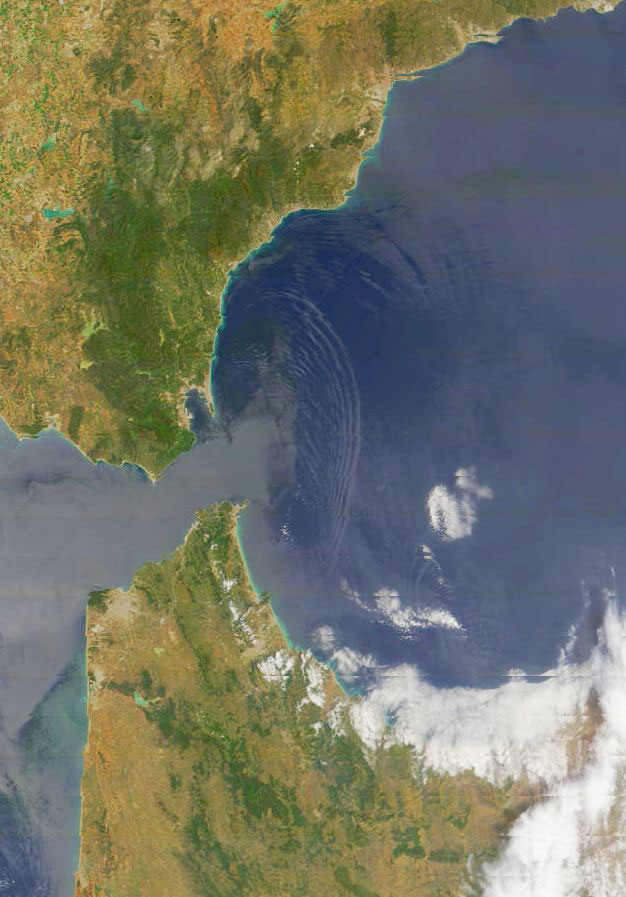
\includegraphics[width = 4cm]{images/internalwavesgibraltar.jpg}
    \caption{Internal waves in the Eastern Strait of Gibraltar. Source: \cite{eumetsat_2017}}
    \label{fig:gibraltar}
\end{figure}

A solution of (\ref{benjaminono}) has the form \cite{chen1979}

\begin{equation}
    u(x,t) = i\sum_{n=1}^N \Big ( \frac{1}{x - z_n(t)} - \frac{1}{x - z_n^\ast (t)} \Big )\;,
\end{equation}

whose poles satisfy the complex Calogero-Moser equations of motion

\begin{equation}
    \ddot z_n(t) = 8 \sum_{m=1,\;m \neq n}^N \frac{1}{(z_n(t) - z_m(t))^3}\;.
\end{equation}

More generally, the following holds \cite{philip2019soliton}.

\begin{thm}
Let $\alpha(x)$ be a special Lax function. The meromorphic functions 

\begin{equation}\label{solitonequation}
    u(x,t) = \sum_{j=1}^N \alpha (x - x_j) - \sum_{n=1}^M \alpha (x - z_n) - i\omega x\;,
\end{equation}

for arbitrary $N$ and $M$ form a class of solutions to equations of Benjamin-Ono type (the equation (\ref{benjaminono}) itself in the rational case with $\omega = 0$, see \cite{philip2019soliton} for the other cases) if and only if their poles $\{x_j\}$ and $\{z_n\}$ satisfy the system of equations

\begin{subequations}
\begin{align}[left=\empheqlbrace]
\dot x_j &= - \sum_{k=1,\;k \neq j}^N \alpha(x_j - x_k) + \sum_{n = 1}^M \alpha(x_j - z_n) + \lambda + i\omega x_j\;,\\
\dot z_n &= \sum_{m=1,\;m \neq n}^M \alpha(z_n - z_m) - \sum_{l = 1}^N \alpha(z_n - x_l) + \lambda + i\omega z_n\;,
\end{align}
\end{subequations}

where $\lambda$ and $\omega$ are constants. 
\end{thm}

We can operate a finite-dimensional reduction of such infinite-dimensional systems. Given a solution of that system of the form $u(x,t)$ we can consider a discretization $u(x; \{z_n\})$ so that the time dependence of $u$ is reduced to $M$ complex parameters $z_n (t)$, with $n = 1, 2,..., M$ with known time dependence. We call $u(x, \{z_n(t)\})$ for $n = 1, ..., M$ an $M$-soliton solution \cite{abanov2011}. 

\section{General method}\label{sec:general}
Consider $N$ complex canonical coordinates $x_j = q_j, \dot x_j = p_j \in \mathbb{C}$ and $M$ canonical coordinates $z_n, \dot z_n \in \mathbb{C}$ and their respective Hamiltonians

\begin{subequations}
\begin{align}
    \mathcal{H} &= \frac{1}{2}\sum_j ({\dot x_j}^2 + \omega^2 x_j^2) + \sum_{j < k} V(x_j - x_k), \\
    \mathcal{H'} &= \frac{1}{2}\sum_n ({\dot z_n}^2 + \omega^2 z_n^2) + \sum_{n < m} V(z_n - z_m)\;,
\end{align}
\end{subequations}

with 

\[V(x) = \left \{ \begin{array}{cc}
{g^2}/{x^2}  & \textnormal{(I)}\\
{g^2a^2}/{\sin^2{ax}}  & \textnormal{(II)}\\
{g^2a^2}/{\sinh^2{ax}} & \textnormal{(III)}
\end{array}
\right.\]

In the literature, $\{x_j\}$ is often called the \textit{principal system} and $\{z_n\}$ the \textit{auxiliary system} or the \textit{dual Calogero-Moser system}. From now on we write the special Lax function as $i\alpha(x)$, with $\alpha(x) = g/x$, $ga/\sin{ax}$ or $ga/\sinh{ax}$, which is real on the real axis. Then a subset of the solutions to each system can be connected by a Bäcklund transformation of the form

\begin{subequations}
\begin{align}[left=\empheqlbrace]
\dot x_j &= - i\sum_{k=1,\;k \neq j}^N \alpha(x_j - x_k) + i\sum_{n = 1}^M \alpha(x_j - z_n) + i\omega x_j \label{soliton1}\;,\\
\dot z_n &= i\sum_{m=1,\;m \neq n}^M \alpha(z_n - z_m) - i\sum_{l = 1}^N \alpha(z_n - x_l) + i\omega z_n\label{soliton1b}\;.
\end{align}
\end{subequations}

\begin{obs}
Taking the time derivative of (\ref{soliton1}) and (\ref{soliton1b}) and using (\ref{soliton1}) and (\ref{soliton1b}) again, we obtain the decoupled systems of second-order ODEs

\begin{subequations}
\begin{align}
    \ddot x_j &= - \frac{\partial }{\partial x_j} \sum_{i = 1,\; i \neq j}^N V(x_i - x_j) - \omega^2 x_j \\
    \ddot z_n &= - \frac{\partial }{\partial z_n} \sum_{m = 1,\; m \neq n}^M V(z_m - z_n) - \omega^2 z_n\;,
\end{align}
\end{subequations}

that are the equations of motion of the two systems considered. 
\end{obs}

For $M < N$, the principal system is reduced via the Bäcklund transformation into a system with fewer degrees of freedom. \\
If $x_j, p_j = \dot x_j \in \mathbb{R} \;\forall j$ (real reduction), (\ref{soliton1}) may be split into two equations concerning separately real and imaginary parts:

\begin{subequations}
\begin{align}[left=\empheqlbrace]
    \sum_{k=1,\;k \neq j}^N \alpha (x_j - x_k) &= \sum_{n=1}^M \operatorname{Re}{\alpha(x_j - z_n)} + \omega x_j \label{soliton2}\;, \\
    \dot x_j &= - \sum_{n = 1}^M \operatorname{Im}{\alpha(x_j - z_n)} \label{soliton3}\;.
\end{align}
\end{subequations}

For $M$ given initial conditions $\{z_n(0)\}$, one can find both $N$ real positions $\{x_j(0)\}$ solving numerically (\ref{soliton2}), and the corresponding real momenta $\{\dot x_j(0)\}$ using (\ref{soliton3}) \cite{philip2019soliton}. Then, the evolutions of the soliton solutions are completely and independently determined by the Olshanetsky-Perelomov projection method, due to the eigenvalues' invariance.

\section{1-soliton solutions for eCM}
Let us apply the general method to the special case of the rational potential with external harmonic potential (eCM). For $M = 1$ the Bäcklund transformations read

\begin{subequations}
\begin{align}[left=\empheqlbrace]
\dot x_j &= -ig \sum_{k=1,\;k \neq j}^N \frac{1}{(x_j - x_k)} + ig \frac{1}{(x_j - z)} + i\omega x_j \label{soliton4}\;,\\
\dot z &= - ig \sum_{l=1}^N \frac{1}{(z - x_l)} + i\omega z\;.
\end{align}
\end{subequations}

Separating (\ref{soliton4}) into its real and imaginary parts, we get

\begin{subequations}
\begin{align}[left=\empheqlbrace]
    \omega x_j &= g\sum_{k=1,\;k \neq j}^N \frac{1}{x_j - x_k} - g \operatorname{Re}{\frac{1}{x_j - z}} \label{soliton5}\;, \\
    \dot x_j &= - g \operatorname{Im}{\frac{1}{x_j - z}} \label{soliton6}\;.
\end{align}
\end{subequations}

Solving numerically (\ref{soliton5}) for a given initial condition $z(0)$, we find $N$ real positions $\{x_j(0)\}$, and then the corresponding real momenta $\{\dot x_j(0)\}$ using (\ref{soliton6}). The evolutions of the soliton solutions are determined by the Olshanetsky-Perelomov procedure: $\{x_j(t)\}$ and $\{z(t)\}$ are given respectively by the eigenvalues of the matrix

\begin{equation}
    X_{jk} (t) = \delta_{jk} \Big (\dot x_j(0)\frac{\sin{\omega t}}{\omega} + x_j (0)\cos{\omega t} \Big ) + (1 - \delta_{jk}) ig \frac{\sin{\omega t}}{\omega(x_j(0) - x_k(0))}\;,
\end{equation}

and by the equation of motion

\begin{equation}
    z(t) = \Big (\dot z(0)\frac{\sin{\omega t}}{\omega} + z(0)\cos{\omega t} \Big ) \;.
\end{equation}

Solving the system numerically\footnote{We use the function \texttt{FindRoot} in Wolfram Mathematica 13.}, we get the worldlines for the real system.

\begin{figure}[H]
    \centering
    \worldlines{data/fig3_2.csv}{10}{12cm}{7.5cm}
    \caption{Worldlines of the real $\textnormal{I}^+$ system for $N = 10$ particles, with $\omega = g = 1$ and initial value $z(0) = 1 + i$.}
    \label{fig:my_label}
\end{figure}

The soliton wave propagates along the real axis in coordination with the complex orbit $z(t)$. The soliton wave appears to propagate with constant speed (the shifts appear to be regularly spaced in time). The soliton excitation corresponds to the upward or downward shifts in the worldlines.  

\begin{figure}[H]
\centering
\begin{subfigure}{.49\textwidth}
  \centering
  \worldlines{data/fig3_3a.csv}{10}{\linewidth}{0.75\linewidth}
  \caption{}
  \label{fig:sub1}
\end{subfigure}%
\begin{subfigure}{.49\textwidth}
  \centering
  \worldlines{data/fig3_3b.csv}{10}{\linewidth}{0.75\linewidth}
  \caption{}
  \label{fig:sub2}
\end{subfigure}
\caption{Worldlines of the real $\textnormal{I}^+$ system for $N = 10$ particles, with $\omega = g = 1$ and initial values $z(0) = 1.2 + 0.3i$ for \ref{fig:sub1} and $z(0) = 2.8 + 2.4i$ for \ref{fig:sub2}.}
\label{fig:test}
\end{figure}

In Figure~\ref{fig:test} we can observe that if $z(0)$ is closer to the real axis, it yields a tighter orbit and more pronounced wave, while $z(0)$ farther gives the opposite behaviour, as confirmed by \cite{philip2019soliton}.

\section{$M$-soliton solutions for eCM}
We can apply the general method to the rational potential with external harmonic potential (eCM) for a generic $M < N$:

\begin{subequations}
\begin{align}[left=\empheqlbrace]
\dot x_j &= -ig \sum_{k=1,\;k \neq j}^N \frac{1}{(x_j - x_k)} + ig \sum_{n = 1}^M \frac{1}{(x_j - z_n)} + i\omega x_j \label{soliton7}\;,\\
\dot z_n &= ig \sum_{m=1,\;m\neq n}^M \frac{1}{z_n - z_m} - ig \sum_{l=1}^N \frac{1}{(z_n - x_l)} + i\omega z_n\;.
\end{align}
\end{subequations}

Separating (\ref{soliton7}) into its real and imaginary parts, we get

\begin{subequations}
\begin{align}[left=\empheqlbrace]
    \omega x_j &= g\sum_{k=1,\;k \neq j}^N \frac{1}{x_j - x_k} - g \sum_{n=1}^M\operatorname{Re}{\frac{1}{x_j - z_n}} \label{soliton8}\;, \\
    \dot x_j &= - g \sum_{n=1}^M\operatorname{Im}{\frac{1}{x_j - z_n}} \label{soliton9}\;.
\end{align}
\end{subequations}

Solving numerically (\ref{soliton8}) for $M$ given initial conditions $\{z_n(0)\}$, we find $N$ real positions $\{x_j(0)\}$, and then the corresponding real momenta $\{\dot x_j(0)\}$ using (\ref{soliton9}). The evolutions of the soliton solutions $\{x_j(t)\}$ and $\{z_n(t)\}$ are given by the eigenvalues of the matrices

\begin{subequations}
\begin{align}
    X_{jk} (t) &= \delta_{jk} \Big (\dot x_j(0)\frac{\sin{\omega t}}{\omega} + x_j (0)\cos{\omega t} \Big ) \nonumber\\ &\quad + (1 - \delta_{jk}) ig \frac{\sin{\omega t}}{\omega(x_j(0) - x_k(0))}\;, \\
    Z_{nm} (t) &= \delta_{nm} \Big (\dot z_n(0)\frac{\sin{\omega t}}{\omega} + z_n (0)\cos{\omega t} \Big ) \nonumber\\ &\quad + (1 - \delta_{nm}) ig \frac{\sin{\omega t}}{\omega(z_n(0) - z_m(0))}\;.
\end{align}
\end{subequations}

We present the results obtained numerically for $M = 2$. 

\begin{figure}[H]
\centering
\begin{subfigure}{.49\textwidth}
  \centering
  \worldlines{data/fig3_4a.csv}{6}{\linewidth}{0.75\linewidth}
  \caption{}
  \label{2soliton61}
\end{subfigure}%
\begin{subfigure}{.49\textwidth}
  \centering
  \worldlines{data/fig3_4b.csv}{6}{\linewidth}{0.75\linewidth}
  \caption{}
  \label{2soliton62}
\end{subfigure}
\caption{Worldlines of the real $\textnormal{I}^+$ system for $N = 6$ particles, with $\omega = g = 1$ and initial values $z_1(0) = -1.1 + 0.5i, z_2(0) = 0.1 -2i$ for \ref{2soliton61} and $z_1(0) = -1.1 + 0.5i, z_2(0) = 0.1 - i$ for \ref{2soliton62}.}
\end{figure}

For $M > 1$, we can note the effects of interaction between multiple solitons. The trajectories are deformed more or less significantly depending on the degrees of freedom of the dual system and the initial conditions.  

\begin{figure}[H]
\centering
\begin{subfigure}{.49\textwidth}
  \centering
  \worldlines{data/fig3_5a.csv}{6}{\linewidth}{0.75\linewidth}
  \caption{}
  \label{2soliton63}
\end{subfigure}%
\begin{subfigure}{.49\textwidth}
  \centering
  \worldlines{data/fig3_5b.csv}{6}{\linewidth}{0.75\linewidth}
  \caption{}
  \label{2soliton64}
\end{subfigure}
\caption{Worldlines of the real $\textnormal{I}^+$ system for $N = 6$ particles, with $\omega = g = 1$ and initial values $z_1(0) = 0.1 + 0.5i, z_2(0) = 0.1 -0.9i$ for \ref{2soliton63} and $z_1(0) = 0.1 + 0.5i, z_2(0) = 0.1 - 0.1i$ for \ref{2soliton64}.}
\end{figure}

\begin{figure}[H]
    \centering
    \worldlines{data/fig3_6.csv}{10}{12cm}{7.5cm}
    \caption{Worldlines of the real $\textnormal{I}^+$ system for $N = 10$ particles, with $\omega = g = 1$ and initial values $z_1(0) = 0.1 + 0.5i, z_2(0) = 0.1 - i$.}
    \label{figsoliton10}
\end{figure}

\begin{obs}
As noted by \cite{abanov2011} and reported in \cite{kulkarni2017, philip2019soliton}, soliton solutions to the rational CM system correspond to extremal conditions of an electrostatic energy function $E$. In fact, considering the Coulomb potential $V(x_j - z_n) = \ln{|x_j - z_n|} = \frac{1}{2}\big[\ln{(x_j - z_n)} + \ln{(x_j - \bar z_n)}\big]$, we get

\begin{equation}
    \frac{\partial V(x_j - z_n)}{\partial x_j} = \frac{1}{2} \Big ( \frac{1}{x_j - z_n} + \frac{1}{x_j - \bar z_n} \Big ) = \operatorname{Re}{\frac{1}{x_j - z_n}}\;.
\end{equation}

Then, given $E$ the potential of the system

\begin{equation}
    E = \sum_{j=1}^N \frac{\omega x_j^2}{2} - g \sum_{1 \leq j < k \leq N} \ln{|x_j - x_k|} + \frac{g}{2} \sum_{j = 1}^N \sum_{n=1}^M \ln{|x_j - z_n|^2}\;,
\end{equation}

it follows

\begin{equation}
    \frac{\partial E}{\partial x_j} = \omega x_j - g \sum_{k=1,\;k \neq j}^N \frac{1}{x_j - x_k} + g\sum_{n=1}^M \operatorname{Re}{\frac{1}{x_j - z_n}}\;.
\end{equation}

Hence, equation (\ref{soliton8}) can be derived from the extremal condition 

\begin{equation}
    \frac{\partial E}{\partial x_j} = 0\;.
\end{equation}

In this view, the positive charges $\{z_n\}$ interact with the negative charges $\{x_j\}$ on the line, inducing the soliton wave. 
\end{obs}

\section{Conclusions}
In Section~\ref{sec:general} we described, following \cite{philip2019soliton}, a general method to find soliton solutions to a variety of systems of Calogero-Moser type (in particular, systems of class I, II, III and $\textnormal{I}^+$). The method takes advantage of the unified description of these systems in terms of their Bäcklund transformations, which depend on a single special Lax function $\alpha(x)$, as seen in Chapter~\ref{ch:cm}. We saw that Bäcklund transformations and $M$-soliton solutions reduce the number of degrees of freedom of the systems considered: it is sufficient to specify $M$ initial conditions for the dual $M$-dimensional system $\{z_n\}$ to determine the dynamics of the real CM system with $N$ degrees of freedom, for the generic $N$. Finally, we presented some numerical examples of $M$-soliton solutions for $M = 1, 2$ for the rational CM system with external harmonic potential (eCM or $\textnormal{I}^+$).  

%\appendix
%\chapter{Appendix}
%\input{chapters/appendix}

\renewcommand{\bibname}{References}
\cleardoublepage\phantomsection
\addcontentsline{toc}{chapter}{References}

\nocite{*}
\bibliographystyle{ieeetr}
\bibliography{references}

\end{document}